\documentclass[tikz,border=0pt]{standalone}
\usepackage{libertinus}
\usepackage{tikz}

\begin{document}

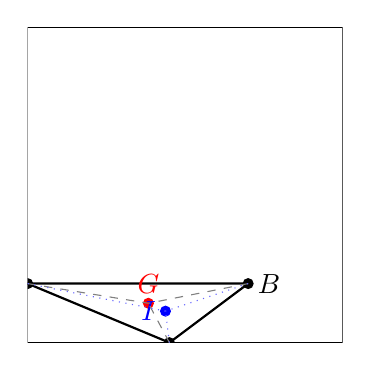
\begin{tikzpicture}[
    x=0.05cm,
    y=0.05cm,
]

% Shift to keep all points positive
\begin{scope}[shift={(36,0)}]

% Clip to 4cm � 4cm = 80 � 80 units
\clip (0,0) rectangle (80,80);

% Draw boundary box
\draw[black] (0,0) rectangle (80,80);

% Vertices
\coordinate (A) at (36,0);
\coordinate (B) at (56,15);
\coordinate (C) at (0,15);

% Centroid
\coordinate (G) at (92/3,10);

% Incenter
\coordinate (I) at (35,8);

% Triangle
\draw[thick] (A)--(B)--(C)--cycle;

% Points
\fill (A) circle (2pt) node[below] {$A$};
\fill (B) circle (2pt) node[right] {$B$};
\fill (C) circle (2pt) node[left] {$C$};

% Centroid and Incenter
\fill[red] (G) circle (2pt) node[above] {$G$};
\fill[blue] (I) circle (2pt) node[left] {$I$};

% Optional lines
\draw[dashed,gray] (A)--(G);
\draw[dashed,gray] (B)--(G);
\draw[dashed,gray] (C)--(G);

\draw[dotted,blue!60] (A)--(I);
\draw[dotted,blue!60] (B)--(I);
\draw[dotted,blue!60] (C)--(I);

\end{scope}

\end{tikzpicture}

\end{document}
